%!TEX root = ./main.tex
%
% This file is part of the i10 thesis template developed and used by the
% Media Computing Group at RWTH Aachen University.
% The current version of this template can be obtained at
% <http://www.media.informatik.rwth-aachen.de/karrer.html>.

\chapter{Related work}
\label{relatedwork}

In this chapter we give an overview of related work and research in the the fields of under water navigation systems. 
It is divided into three parts.
First we give an overview of currently used technology used for underwater position tracking and the issues in comparison with common GPS.
Second it covers existing systems which incorporate position tracking and underwater feedback today and third research regarding several feedback modalities. 

It is commonly known that radio signals do not propagate underwater.
Currently state of the art solutions consists of large and expensive inertial measurement units. 
Those are for example used in submarines and use the last known position in combination with military grade accelerometer and diving depth to interpolate the current location \citep{meyer}.

\mnote{Inertial Data Fusion}
\cite{Rossi_Performance} presented a data fusion algorithm for inertial navigation with focus on performance.
It is based on the idea of data fusion which measures and combines values from several inertial sensors.

\mnote{Acoustic GPS}
\cite{Taraldsen_UnderwaterGPS} technology relies on acoustic waves as an analogy to the GPS radio waves.
They discuss different approaches of Dilution Of Precision (DOP) which differ from the classical GPS setting.
Using statistical methods, they estimate the accuracy of positioning and try to correct errors.


\section{Underwater Navigation Systems}

\mnote{Navimate}
\cite{navimate} developed Navimate which uses a floating radio antenna for GPS and several underwater transducers to communicate with a wrist-worn device via acoustic signals. 
The device receives the signals and uses the information of the GPS and the transducers to determine its location and presents the information on the screen. 

\mnote{NavDive}
\cite{navdive} built NavDive which uses a floating GPS receiver wired to a mobile receiver held by the diver. 
It shows the direction to previously set locations and positional information in text form. 
A desktop application lets the user inspect their diving path and add landmarks for locations of interest.

\mnote{Ariadna Tech}
\cite{ariadna} developed a system which uses an initial GPS location from the wrist unit before submerging and switches to  inertial sensors afterwards.
The sensors track the divers real-time position, speed, heading, and distance information using a navigation transmitter worn on the leg.
It calculates the information in real-time and sends it wireless to to the wrist unit which displays it on screen.

\mnote{WaterLinked}
\cite{waterlinked} uses four hydro acoustic receiver in the water connected to a base station with access to a GPS antenna. 
The tracked object or diver is equipped with a locator which acts as an beacon sending acoustic pulses. 
These acoustic pulses are received be the four hydrophones and analysed with time-of-arrival and the GPS data. This system enables tracking of submerged ROVs and divers but not for the divers themselves.

\begin{figure}
	\centering
	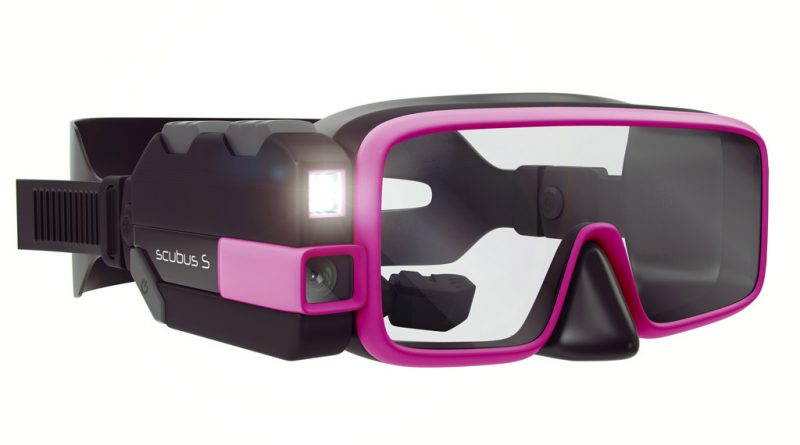
\includegraphics[width=\columnwidth]{images/scubusS.jpg}
	\caption{Scubus S smart diving goggles by Noah Smith.}~\label{fig:scubusS}
	\vspace{-2em}
\end{figure}

\mnote{Scubus S}
\cite{scubus} propose a system similar to featuring a head up display like Google Glass, a LED flash light, and a HD camera. 
All electronics including the battery are integrated into the smart diving goggles.
The crowd funding campaign failed in 2015.
The system is shown in figure~\ref{fig:scubusS} 

\section{Feedback modalities}

\mnote{GentleGuide}
\cite{bosman} built and tested a system using 2 wrist worn vibration devices.
Main findings were that vibration feedback on one wrist is confusing, vibrations are rather a beacon to follow than a correction of one's direction, and that direction is better encoded in the duration of the pulse than the intensity.
Results are promising for non-disruptive, easy learnable, low level-navigation cues.

\mnote{MOVING}
\cite{Kiss:2018:NSM:3173574.3174191} present MOtorbike VIbrational Navigation Guidance, a smart kidney belt for motor cyclists that provides feedback through 12 vibration motors.
Tactile feedback allows distraction free navigation cues which are more reliable and safe than visual based navigation systems used today.

\mnote{HapticHead}
\cite{Kaul_HapticHead} developed HaptiHead a system for intuitive tactile 3D guidance.
The use 20 vibration motors in 3 concentric ellipses around the head to give 3D directional cues in virtual or augmented reality environment.
Vibration performed well compared to direct visual guidance and significantly better than 3D auditory cues.

\mnote{IrukaTact}
IrukaTact by \cite{Chacin_Irukatact} is a a glove which uses water propulsion on the fingertips and a sonar to assist in the location of underwater objects. The sonar detects the topography of the ground and sends the information to the system which uses micro-pumps to convey these information via varying water jets on the fingertips.

\mnote{ThermoVR}
\cite{Peiris_thermoVR} present ThermoVR, a VR headset with five thermal feedback modules. 
The thermal stimulation, hot and cold, were used to increase the immersion and give directional cues.
They found that cold stimuli were perceived significantly better in providing directional feedback.

\cite{Wilson:2011:LHT:1978942.1979316} discovered that cold stimuli are faster to detect and more comfortable for the user. 
They tested different changes of temperature per second and higher rates are better detectable. 
Also producing detectable cold stimuli are more power efficient than warm stimuli.

\cite{Halvey:2012:BCO:2207676.2207779} investigated the environmental effects on thermal feedback recognition. 
They conducted an outdoor study over several month and varying conditions and showed that ambient temperature has a significant effect on the detection and perception of thermal stimuli.
Humidity on the other hand has a negligible effect in mobile interaction. 
This result is supported by \cite{givoni}.

\cite{hirosawa} looked into the effect of room and skin temperature on temperature sensitivity.
Their results show that the threshold values change with the room temperature for both, warm and cold.







































